\chapter{Materials and Methods}
\label{chap:matandmeth}
\section{\Nsm{} Strains Used in This Work}
\begin{table}[h]
\begin{center}
\begin{tabular}{>{\centering}m{4.4cm}m{6.4cm}>{\centering}m{3.1cm}}
\toprule
\textbf{Name} & \centering \textbf{Description} & \textbf{Source}
\tabularnewline
\midrule
MC58 & Wild-Type Strain & \citet{McGuinness1990}
\tabularnewline\noalign{\smallskip}\hline\noalign{\smallskip}
$\Delta$norB::spc$^\textrm{r}$\nomenclature{spc$^\textrm{r}$}{Spectinomycin resistance} & Wild-Type with insertion of spectinomycin resistance cassette into \textit{norB} gene & \citet{Heurlier2008}
\tabularnewline\noalign{\smallskip}\hline\noalign{\smallskip}
$\Delta$nsrR::spc$^\textrm{r}$ & Wild-Type with insertion of spectinomycin resistance cassette into \textit{nsrR} gene & \citet{Rock2007}
\tabularnewline\noalign{\smallskip}\hline\noalign{\smallskip}
$\Delta$norB::spc$^\textrm{r}$-$\Delta$nsrR::tet$^\textrm{r}$\nomenclature{tet$^\textrm{r}$}{Tetracyclin resistance} & Wild-Type with insertion of spectinomycin resistance cassette into \textit{norB} and insertion of tetracyclin resistance cassette into \textit{nsrR} genes & \citet{Heurlier2008}
\tabularnewline\noalign{\smallskip}\hline\noalign{\smallskip}
$\Delta$aniA::spc$^\textrm{r}$-$\Delta$nsrR::tet$^\textrm{r}$ & Wild-Type with insertion of spectinomycin resistance cassette into \textit{aniA} and insertion of tetracyclin resistance cassette into \textit{nsrR} genes & \citet{Heurlier2008}
\tabularnewline
\bottomrule
\end{tabular} 
\end{center}
\caption{Bacterial strains and sources
\label{tab:bacterial-strains}}
\end{table}

\section{Culturing \Nsm{}}
\subsection{Growth of \Nsm{}}
\Nm{} strains were grown on plates on Columbia Agar Base (CAB)\nomenclature{CAB}{Columbia Agar Base} with defibrinated horse blood, and in liquid culture in M\"uller-Hinton Broth (MHB)\nomenclature{MHB}{M\"uller-Hinton Broth}.

Plates were prepared by adding horse blood to a final concentration of 5\% to molten agar, and poured into plastic petri dishes. After streaking with \Nm{} the plates were incubated at 37\textdegree C in a 5\% carbon dioxide/air mixture.

Aerobic liquid cultures were grown in 10ml MHB with 1\% NaHCO$_\textrm{3}$ in plastic sterilin tubes, and incubated at 37\textdegree C at 200rpm\nomenclature{rpm}{Revolutions Per Minute}. Microaerobic cultures were suspended in 20ml MHB, 1\% NaHCO$_\textrm{3}$ in plastic sterilin tubes, incubated at 37\textdegree C at 100rpm.

\subsection{Preparation of Antibiotic Selective Media}
Liquid stock solutions of required antibiotics were either added directly to liquid culture, or, if growing on plates, to the molten agar when also adding horse blood. The final concentrations of antibiotics are given in Table \ref{tab:antibiotic-concs}.

\begin{table}[here]
\begin{center}
\begin{tabular}{cc}
\toprule
\textbf{Antibiotic} & \textbf{Final concentration ($\mu$g/ml)} \\
\midrule
Spectinomycin & 50 \\
Tetracyclin & 2.5 \\
Chloramphenicol & 50 \\
\bottomrule
\end{tabular} 
\end{center}
\caption{Final antibiotic concentrations
\label{tab:antibiotic-concs}}
\end{table}

\subsection{Preparation of Frozen Bacterial Stocks}
Bacteria were grown in liquid culture until late log phase prior to harvesting. Liquid cultures were then centrifuged at 4000g for 15 minutes, and the pellet was then resuspended in a 25\% glycerol, 25\% water and 50\% MHB, all of which had been autoclaved beforehand. The bacterial stocks were then frozen at $-80$\textdegree C.

\subsection{Streaking Plates for OD to CFU Ratio Calculation}
Bacterial cultures were grown overnight and then transferred into aerobic liquid culture and samples taken throughout the day to obtain a range of different optical densities. The optical density was recorded at 600nm, and each sample was serially diluted to the following levels: $10^{-5}$, $10^{-6}$ and $10^{-7}$. 100$\mu$l of each of these dilutions was plated on a fresh blood agar plate and left to grow overnight. The following morning the number of colonies on each plate was counted and used to create a standard curve for Optical Density\nomenclature{OD}{Optical Density} to Colony Forming Units\nomenclature{CFU}{Colony Forming Units}.

\section{Measuring Oxygen Concentration}
Oxygen concentration in respiring cultures was measured using a Clark electrode \cite{Clark1953} from Rank Brothers, Cambridge, UK. This electrode has a silver anode and a platinum cathode using a saturated potassium chloride solution as electrolyte. The electrode is set at the bottom of a ~7ml reaction chamber separated from its contents by a thin Teflon membrane. This membrane is permeable to dissolved oxygen, and is reduced by the electrode producing a measurable electrical current. The reaction chamber is maintained at $37$\textdegree C by an attached water bath.
When performing experiments, 5ml of culture is added to the reaction chamber, which is stirred by use of a magnetic flea, and the chamber covered with a plastic stopper. The stopper has a number of holes through which the NO probe, or Hamilton syringe can be inserted. Data is collected by attaching the electrode to an external data logger (Pico ADC20, Pico Technology).

\subsection{Calibration of Oxygen Electrode}
Calibration of the oxygen electrode assumes that anaerobic water will not produce any measurable current at the electrode. Oxygen saturated water contains 210$\mu$M Oxygen (ref needed). 5ml of ultra pure water was added to the electrode chamber, and then aerated to saturation by use of a pasteur pipette. The maximum value recorded by the data logger then corresponds to a concentration of 210$\mu$M Oxygen, with the relationship between mV as recorded against concentration being linear.

\section{Measuring Nitric Oxide Concentration}
Nitric Oxide concentration was measured using a Nitric Oxide probe (ISO-NOP, World Precision Instruments) connected to a Nitric Oxide Meter (ISO-NO mkII, World Precision Instruments). This is also a Clark type electrode, contained within a steel sleeve with a semi-permeable membrane separating the working electrode from the system being measured\cite{Liu2005,Bedioui2003,Serpe2007}. The NO probe is inserted through one of the holes in the plastic lid of the reaction chamber of the oxygen electrode assembly. The tip of the electrode should be immersed in the culture, with care being taken not to trap any air bubbles on the surface of the probe. The sensor is also attached to the same data logger as above. In this way both Oxygen and Nitric Oxide concentrations can be measured in parallel.

\subsection{Calibration of Nitric Oxide Electrode}
Calibration of the nitric oxide electrode relies on adding known quantities of Nitric Oxide to the electrode chamber. Sodium Nitrite will liberate Nitric Oxide with a 1:1 ratio when added to a solution of excess Potassium Iodide and Sulfuric acid based on the following reaction:

\begin{equation}
2\mathrm{NaNO}_2 + 2\mathrm{KI} + 2 \mathrm{H}_2\mathrm{SO}_4 \longrightarrow 2\mathrm{NO} + \mathrm{I}_2 + 2\mathrm{H}_2\mathrm{O} + 2\mathrm{Na}_2\mathrm{SO}_4
\end{equation}
5ml of 0.1M Potassium Iodide/Sulfuric Acid was added to the electrode chamber and allowed to stabilise. Then, increasing concentrations of Sodium Nitrite solution were successively added to produce a standard curve of Nitric Oxide concentration to recorded electrode mV. The volume and concentrations of Soduim Nitrite added to the electrode chamber are detailed in Table \ref{tab:sodiumnitrite}.

\begin{table}[here]
\begin{center}
\begin{tabular}{ccc}
\toprule
\multicolumn{2}{c}{$\mathbf{NaNO}_2$} & \textbf{NO} \\
\textbf{Concentration ($\mu$M)} & \textbf{Volume ($\mu$l)} & \textbf{Concentration (nM)} \\
\midrule
10 & 50 & 99 \\
100 & 25 & 591 \\
100 & 50 & 1561 \\
\bottomrule
\end{tabular} 
\end{center}
\caption{Sodium Nitrite concentrations used to calibrate ISO-NOP Nitric Oxide sensor.
\label{tab:sodiumnitrite}}
\end{table}

\section{Measuring Nitrite Concentration (Griess Assay)}
Nitrite concentration in liquid culture was determined using the colorimetric assay described by \citet{DonaldNicholas1957}. This reaction is based on chemical diazotization which uses sulfanilamide and \textit{N}-1-napthylethylenediamine dihydrochloride (NED)\nomenclature{NED}{\textit{N}-1-napthylethylenediamine dihydrochloride} under acidic (hydrochloric acid) conditions. Nitrite is converted to nitrous acid under acidic conditions and this then forms a diazonium salt with the sufanilamide. The diazonium salt combines with NED and forms a pink azo dye which can be detected using absorbance spectrophotometry at a wavelength of 540nm. Depending on the expected concentration of nitrite, different sample volumes are used in the assay. The most common sample volume used was $25\mu\textrm{l}$ which allows detection up to around $1\mu\textrm{M}$ nitrite with the following reagent volumes: $875\mu\textrm{l}$ of 1\% sulfanilamide in 1M HCl and $100\mu\textrm{l}$ of 0.02\% NED in 1M HCl. When using different sample volumes, the volume of sulfanilamide was altered such that the volume of sample + sulfanilamide always equalled $900\mu\textrm{l}$. After adding the sample to the reagents, it was left for 20 minutes for the colour to develop, then the absorbance at 540nm was measured and compared to a standard curve.

\section{Nitric Oxide Production}
Solutions of Nitric Oxide were prepared using a method derived from one described by \citet{Aga2008}. The apparatus setup is shown in Figure \ref{fig:nomaker}. 
\begin{figure}
 \centering
 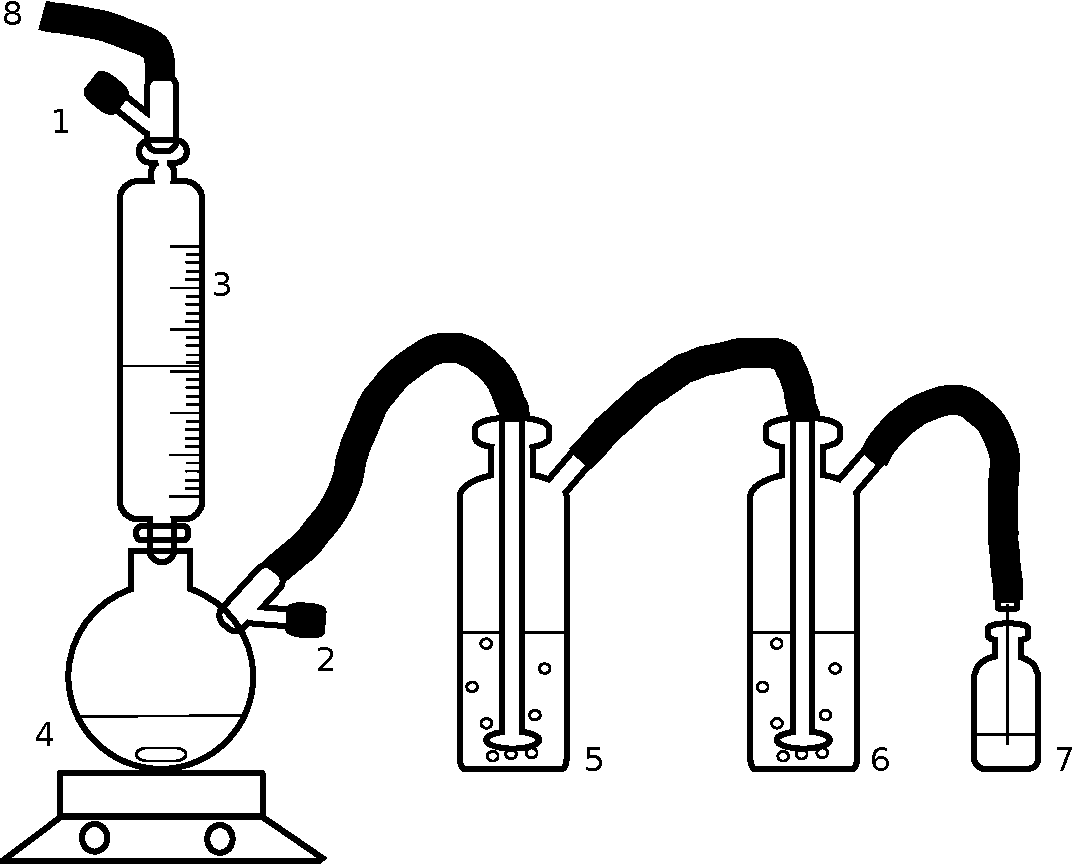
\includegraphics[height=10cm]{./02-materialsmethods/data/drawing.pdf}
 % drawing.pdf: 515x415 pixel, 72dpi, 18.17x14.64 cm, bb=0 0 515 415
 \caption[NO making apparatus.]{{\bf NO making apparatus.} 1 \& 2 - N$_{\textrm{2}}$ release valves. 3 - Pressure equalizing dropping funnel, containing 50ml 4M H$_{\textrm{2}}$SO$_{\textrm{4}}$. 4 - Stirred, round-bottomed flask, containing 200ml 2M NaNO$_{\textrm{2}}$. 5 - Dreschel bottle with sintered bulb, containing \~200ml 1M NaOH ($\frac{2}{3}$ full). 6 - Dreschel bottle with sintered bulb, containing \~200ml dH$_{\textrm{2}}$O ($\frac{2}{3}$ full). 7 - Small glass bottle with rubber septum and needle entry valve, containing dH$_{\textrm{2}}$O $\frac{2}{3}$ full. 8 - To N$_{\textrm{2}}$ gas bottle.
 \label{fig:nomaker}}
\end{figure}
A concentrated solution of Sulfuric acid is added from a pressure-equalizing dropping funnel to a concentrated solution of Sodium Nitrite solution in a stirred, round-bottomed flask. This releases NO gas which passes through a solution of Sodium Hydroxide to neutralise any Sulfuric acid present, then through distilled water to remove any Sodium Hydroxide before finally being bubbled into a collection vessel with a sealed rubber septum containing distilled water. The concentrations of the chemicals used in this preparation are shown in Table \ref{tab:nomakerchem}.
\begin{table}[here]
\begin{center}
\begin{tabular}{ccc}
\toprule
\textbf{Chemical} & \textbf{Volume (ml)} & \textbf{Concentration (M)} \\
\midrule
$\textrm{NaNO}_2$ & 200 & 2 \\
$\textrm{H}_2\textrm{SO}_4$ & 50 & 4 \\
NaOH & 200 & 1 \\
\bottomrule
\end{tabular} 
\end{center}
\caption{Chemicals needed for preparation of Nitric Oxide solution.
\label{tab:nomakerchem}}
\end{table}\\
The system should be set up in a fume cupboard as shown in Figure \ref{fig:nomaker} and sparged with $\textrm{N}_2$ gas for 15 minutes (the dropping funnel will allow gas to pass into the round bottomed flask even when the bottom valve is closed). The $\textrm{H}_2\textrm{SO}_4$ should be sparged separately. Valve 2 should be left open at all times. After sparging close valve 1 and then add the Sulfuric acid dropwise from the dropping funnel. Brown gas will start to bubble through to the collection vessel. This apparatus should produce enough NO gas to saturate several small (10ml) collection vessels which should have the needle removed and be sealed once saturated. Once all the Sulfuric acid has been added leave the reaction to finish which could take 1-2 hours. Before disassembly sparge the apparatus with $\textrm{N}_2$ gas to remove residual NO gas.

The eventual concentration of NO in the solution will vary depending on the temperature, but at 25\textdegree{}C in pure water the concentration will be between 1.88 and 1.96 mM\cite{Aga2008,Cole2008}.

\section{Solving Ordinary Differential Equations}
The model equations (given in Chapter \ref{chap:model} [\nameref{chap:model}]) are solved in parallel using the common $\mathrm{6}^\mathrm{th}$ order Runge-Kutta-Fehlberg algorithm for integrating ordinary differential equations \cite{Butcher2003}. Adaptive step-sizes were implemented using the Cash-Karp method\cite{Cash1990}. The adaptive step size system was required as it prevented the introduction of systemic numerical instabilities.

The parameter estimation system and ODE solver were a bespoke implementation written in Java. The Runge-Kutta algorithm was modified from that found in Numerical Recipes in C\cite{Press1992}. I decided to write a custom implementation rather than using off the shelf systems for solving ODEs and parameter estimation as I wanted the greatest flexibility in how I integrated the two techniques, and it allowed me to quickly and easily tailor the code to my needs. Initially I tried using COPASI \cite{Hoops2006}, however at that time it had limitations that I could not overcome, such as bulk addition of components at arbitrary time-points.

The implementation of the model has no constraints on respiratory substrate concentration, thus allows the altering of these concentrations whilst solving the equations, however changes to substrate concentration have to be made programmatically to inform the model of the change (\texttt{if (t == 50) then NO\_conc += 20;}). This ability means that the switch between aerobic and anaerobic respiration can be examined synthetically, and the model is also capable of simulating how the respiratory system responds to addition of substrates such as Nitric Oxide. This ability was an absolute requirement, as in order to fully parametrise the model it was necessary to isolate sections of the model, which required adding aliquots of respiratory substrate during respiration.

\section{Parameter Estimation}
Estimating the parameter values for the components in the mathematical model involved comparing the biological results with those produced by solving the ODEs and adjusting the parameter values to minimise the difference between the two results. The different methods for parameter estimation that I investigated are detailed in Chapter \ref{chap:paramest} [\nameref{chap:paramest}].